% Project:     DNS resolver
% @file        doc/documentation.tex
% @date        14.11.2023
% 
% @brief Documentation file
%
% @author Adam Ližičiar <xlizic00@stud.fit.vutbr.cz>

\documentclass[a4paper, 11pt]{article}

\usepackage[slovak]{babel}
\usepackage[utf8]{inputenc}
\usepackage[left=2cm, top=3cm, text={17cm, 24cm}]{geometry}
\usepackage{times}
\usepackage{verbatim}
\usepackage{enumitem}
\usepackage{graphicx}
\usepackage[unicode]{hyperref}
\hypersetup{
    colorlinks=true,
    linkcolor=black,
    urlcolor=blue, 
    citecolor=blue
}

\begin{document}

	%%%%% Titulná stránka %%%%%
	\begin{titlepage}
		\begin{center}
			
\includegraphics[width=0.77\linewidth]{res/logo_FIT.pdf} \\

			\vspace{\stretch{0.382}}

			\scalebox{2}{\Huge{Manuál}} \\
			\LARGE{DNS Resolver} \\
			\vspace{\stretch{0.618}}
		\end{center}

		\begin{minipage}[b]{0.4 \textwidth}
			\raggedright
			{\Large \today}
		\end{minipage}
		\hfill
		\begin{minipage}[b]{0.6 \textwidth}
			\raggedleft
			\Large
			Adam Ližičiar (xlizic00)\\
		\end{minipage}		
	\end{titlepage}

	%%%%% Obsah %%%%%
	\pagenumbering{roman}
	\setcounter{page}{1}
	\tableofcontents
	\clearpage

	\pagenumbering{arabic}
	\setcounter{page}{1}
	
	%%%%% Úvod %%%%%
	\section{Úvod}
	DNS (Domain Name System) resolver je~kľúčovou súčasťou internetovej infraštruktúry, umožňujúcou prevod ľudom čitateľných doménových mien (ako je~napríklad \texttt{www.fit.vut.cz}) na~IP adresy, ktoré~ ~používané pre~sieťovú komunikáciu. Tento dokument poskytuje prehľad funkcií a~implementácie programu \texttt{dns}, ktorý bol navrhnutý na~zasielanie dotazov na~DNS servery a~na~zobrazenie prijatých odpovedí na~štandartnom výstupe.
	\subsection{Charakteristika DNS}
	DNS je~hierarchický a~decentralizovaný systém, ktorý~umožňuje užívateľom na~internete nájsť webové stránky a~iné služby prostredníctvom ľudom čitateľných názvov, tzv.~doménových mien. DNS servery sú~zodpovedné za~prevod týchto názvov na~IP adresy (alebo naopak), ktoré sú~nevyhnutné pre~nadviazanie sieťového spojenia.
	\subsection{Funkcie a účel programu DNS resolver}
	Program \texttt{dns} je nástroj navrhnutý na~zasielanie dotazov na~DNS servery a~analýzu prijatých odpovedí. Umožňuje používateľom vykonávať dotazy v~čitelné podobe a~poskytuje informácie o~odpovediach od~DNS serverov. Priamo v~programe je~implementované zostavenie a~odoslanie packetov, bez~potreby nástrojov. Program podporuje komunikáciu pomocou UDP.	

	%%%%% Vytvorenie spustiteľného súboru %%%%%
	\section{Vytvorenie spustiteľného súboru a~automatizácia úloh}
	Prebieha pomocou Makefile na~automatizáciu kompilácie, testovania a~generovania dokumentácie. 
	\begin{itemize}
		\item \texttt{make}: Kompiluje zdrojové súbory projektu a~pomocou kompilátora \texttt{g++} vytvára spustiteľný súbor \texttt{dns}.
		\item \texttt{make run}: Spustí skompilovaný program \texttt{dns} s~preddefinovanými argumentmi, čím~demonštruje jeho funkčnosť.
		\item \texttt{make test}: Spustí testovacie skripty definované v adresári \texttt{tests}, čím overuje správnosť implementácie programu.
		\item \texttt{make doc}: Generuje dokumentáciu projektu vo~formáte PDF pomocou nástroja \texttt{pdflatex}. Všetky súborové operácie sú~vykonávané v~rámci adresára \texttt{doc} a~výsledná dokumentácia je~presunutá do~objektového adresára \texttt{obj} pre~udržanie poriadku.
		\item \texttt{make clean}: Odstráni všetky objektové a~dočasné súbory, ktoré boli vytvorené počas kompilácie, čím~udržuje projektový adresár čistý.
		\item \texttt{make cleanall}: Rozširuje funkcionalitu \texttt{clean} o~odstránenie spustiteľného súboru \texttt{dns}, vygenerovanej dokumentácie v~PDF a~všetkých výstupov z~testov.
	\end{itemize}
	\subsection{Požiadavky na systém}
	Pre~úspešnú kompiláciu a~fungovanie programu je~potrebné zabezpečiť, aby bol program spustený v~operačnom systéme Linux.
	
	%%%%% Spúštanie programu %%%%%
	\section{Spúštanie programu}
	Použitie príkazu \texttt{dns} je~nasledovné:
	\begin{verbatim}
	dns [-h] [-r] [-x] [-6] -s server [-p port] adresa
	\end{verbatim}
	Poradie parametrov je~ľubovoľné, ak nie je nastavená premenná prostredia $POSIXLY_CORRECT$. Každý parameter má~špecifický význam:
	\begin{itemize}
		\item \texttt{-h}: Vypíše vysvetlenie použitia parametrov do~štandartného výstupu. Príklad výstupu je v prílohe \ref{subsection:res_A}
		\item \texttt{-r}: Požadovaná rekurzia (Recursion Desired = 1), inak bez~rekurzie.
		\item \texttt{-x}: Reverzný dotaz namiesto priameho.
		\item \texttt{-6}: Dotaz typu \texttt{AAAA} namiesto preddefinovaného \texttt{A}.
		\item \texttt{-s server}: IP~adresa alebo~doménové meno servera, kam sa má~odoslať dotaz.
		\item \texttt{-p port}: Číslo portu, na~ktorý sa má~odoslať dotaz, preddefinovaný je~53.
		\item \texttt{adresa}: Adresa na zistenie.
	\end{itemize}
	
	\subsection{Príklady výstupov}
	\noindent Odpoveď na príkaz \texttt{./dns -r -s kazi.fit.vutbr.cz www.fit.vut.cz}
	\begin{verbatim}
		Authoritative: Yes, Recursive: Yes, Truncated: No
		Question section (1)
		  www.fit.vut.cz., A, IN
		Answer section (1)
		  www.fit.vut.cz., A, IN, 14400, 147.229.9.26
		Authority section (0)
		Additional section (0)
	\end{verbatim}

	\noindent Odpoveď na príkaz \texttt{./dns -r -6 -s kazi.fit.vutbr.cz www.fit.vut.cz}
	\begin{verbatim}
		Authoritative: Yes, Recursive: Yes, Truncated: No
		Question section (1)
		  www.fit.vut.cz., AAAA, IN
		Answer section (1)
		  www.fit.vut.cz., AAAA, IN, 14400, 2001:67c:1220:809::93e5:91a
		Authority section (0)
		Additional section (0)
	\end{verbatim}

	\noindent Odpoveď na príkaz \texttt{./dns -x -s kazi.fit.vutbr.cz 147.229.9.26}
	\begin{verbatim}
		Authoritative: Yes, Recursive: No, Truncated: No
		Question section (1)
		  26.9.229.147.in-addr.arpa., PTR, IN
		Answer section (1)
		  26.9.229.147.in-addr.arpa., PTR, IN, 14400, www.fit.vut.cz.
		Authority section (4)
		  9.229.147.in-addr.arpa., NS, IN, 14400, rhino.cis.vutbr.cz.
		  9.229.147.in-addr.arpa., NS, IN, 14400, gate.feec.vutbr.cz.
		  9.229.147.in-addr.arpa., NS, IN, 14400, guta.fit.vutbr.cz.
		  9.229.147.in-addr.arpa., NS, IN, 14400, kazi.fit.vutbr.cz.
		Additional section (0)
	\end{verbatim}
	
	%%%%% Analýza a interpretácia výstupov %%%%%
	\section{Analýza a~interpretácia výstupov}
	Táto sekcia rozoberá, čo~možno zistiť vďaka použitiu programu \texttt{dns}.
	\subsection{Rekurzívne a~nerekurzívne dotazy}
	Umožňuje určiť, či sa~má vykonať rekurzívny (-r) alebo nerekurzívny dotaz. Rekurzívne dotazy žiadajú DNS server o~kompletnú odpoveď, zatiaľ čo~nerekurzívne vrátia len informácie, ktoré server už má.
	\subsection{Reverzné dotazy}
	Program umožňuje vykonávať reverzné dotazy (-x), vďaka čomu možno zistiť doménové meno priradené k~erčitej IP adrese.
	\subsection{Typy dotazov AAAA a~A}
	Poskytuje možnosť vykonávať dotazy typu AAAA~(-6) pre~získanie IPv6 adries alebo typu A pre~IPv4 adresy, čo umožňuje flexibilitu v~získavaní sieťových informácií.
	\subsection{Výstupy a~ich interpretácia}
	Výstupy programu sú~prehľadné a informatívne, poskytujú podrobné údaje o~odpovediach DNS serverov. Umožňujú získať dôležité informácie vrátane autoritatívnosti odpovede, rekurzívnych vlastností a~detailov o~dotazovanej adrese.
	\subsection{Využitie výsledkov}
	Na~základe analýzy výsledkov možno získať užitočné informácie pre~sieťovú diagnostiku, administráciu a~plánovanie.

	%%%%% Riešenia problémov a chybové hlášky %%%%%
	\section{Riešenia problémov a chybové hlášky}
	//todo: Bežné problémy a ich riešenia.
	//todo: Vysvetlenie chybových hlášok a kroky k ich odstráneniu.
	
	%%%%% Architektúra programu %%%%%
	\section{Architektúra programu}
	//todo: Stručný popis kľúčových častí programu.

	%%%%% Testovanie programu %%%%%
	\section{Testovanie programu}
	//todo: Postupy a nástroje pre testovanie aplikácie.
	//todo: Príklady testov a ich význam.
	// testy su ok, a treba cakat kvoli zmene TTL.....Obsah databáze DNS se z principů mění a může vypadat z různých míst různě. Např. doporučuji se serveru kazi.fit.vutbr.cz ptát ze sítě FIT. Do jiných sítí mohou být odpovědi jiné. Ukázkové záznamy jsou mimo mou kontrolu a mohou se nepředvídatelně měnit, v průběhu řešení projektu mohou být zrušená, dočasně nedostupná, nově přesměrovaná jinam apod.
	
	Referenční prostředí pro překlad a testování

	Program by měl být přenositelný. Referenční prostředí pro překlad budou servery eva.fit.vutbr.cz a merlin.fit.vutbr.cz (program musí být přeložitelný a funkční na obou systémech). Vlastní testování může probíhat na jiném počítači s nainstalovaným OS GNU/Linux, či FreeBSD, včetně jiných architektur než Intel/AMD, jiných distribucí, jiných verzí knihoven apod. Pokud vyžadujete minimální verzi knihovny (dostupné na serveru merlin a eva), jasně tuto skutečnost označte v dokumentaci a README.

	%error testy testuju, ci na vystupe je chybovy vystup ""

	%%%%% Rozšírenia %%%%%
	\section{Rozšírenia}
	//todo: Aké rozšírenia má program? (podpora viac vecí, chybové kódy, chybové hlášky,...)
	// Errcodes
	// Zadání nespecifikuje, které typy RDATA bychom měli být schopni zpracovávat. Existuje více než 16 typů, ale zadání se zmiňuje pouze o CNAME, A, AAAA. Měl by je program umět zpracovat všechny, nebo jen tyto tři?:::::	Tato funkcionalita je vyžadovaná v zadání. Zpracování dalších, vámi uvedených i typů záznamů z jiných RFC, lze vnímat jako funkcionalitu základní zadání rozšiřující. Pakliže se rozhodnete implementovat funkcionalitu nad rámec zadání, jasně toto rozšíření označte v souboru README a dokumentaci. Vámi implementované rozšíření řádně dokumenujte. Vaše rozhodnutí ve fázi návrhu a implementace řádně dokumentujte a vysvětlete v dokumentaci.
	je tam kontrola na format vstupu argumentov
	// man stranka v src/man/dns.1


	%%%%% Referencie %%%%%
	\section{Referencie}
	//todo: referencie
	https://datatracker.ietf.org/doc/html/rfc1035
	https://datatracker.ietf.org/doc/html/rfc3596

	%%%%% Prílohy %%%%%
	\clearpage
	\section{Prílohy}
	
	\subsection{Výpis \texttt{./dns -h} na~štandartnom výstupe}
	\label{subsection:res_A}

	\begin{figure}[ht]
		\centering
		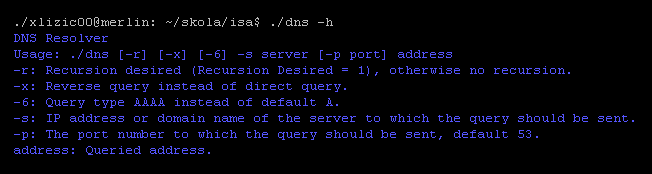
\includegraphics[width=1 \linewidth]{res/A.png}

		\caption{Príklad výstupu \texttt{./dns -h} na~štandartnom výstupe. Príklad bol realizovaný na~serveri \mbox{merlin.fit.vutbr.cz}}
	\end{figure}

\end{document}
